\section{Medidas de relaxamento}
\label{sec:ResRelax}

Após os ensaios de envelhecimento foram realizadas medidas nos dispositivos para verificar a recuperação da degradação infligida a eles. Todos os FPGAs foram deixados desligados e em temperatura ambiente, sendo ligados apenas para realizar as medições.

A Figura \ref{fig:RelaxEstressadas} mostra as curvas das frequências normalizadas ao longo do tempo de relaxamento das placas que foram estressadas termicamente. Nela se vê que os FPGAs da altera recuperaram mais que os da ZedBoard, e que ele apresenta uma tendência de continuar degradando após o fim dos ensaios, enquanto a ZedBoard apresentou uma estabilização na frequência.

\begin{figure}[H]
    \centering
    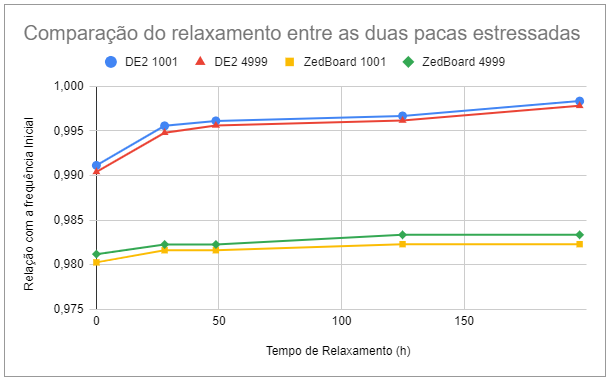
\includegraphics[scale=0.75]{figures/Resultados/RelaxEstressadas}
    \caption{Comparação do relaxamento das duas placas. Fonte: O Autor}
    \label{fig:RelaxEstressadas}
\end{figure}

É demonstrado na Figura \ref{fig:RelaxDE2} como as duas placas DE2 se comportaram ao longo do tempo de relaxamento. É visível que as duas apresentaram semelhança no formato da curva, inclusive alcançando um valor próximo na última medida. 

\begin{figure}[H]
    \centering
    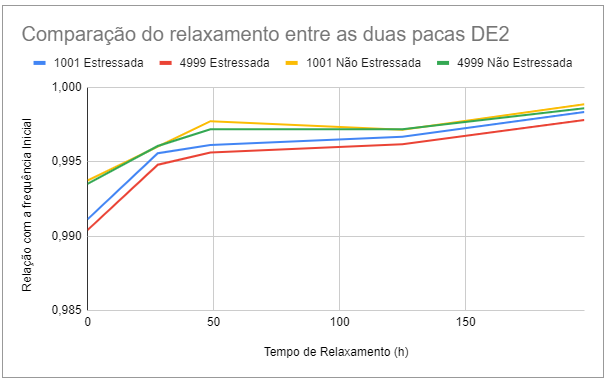
\includegraphics[scale=0.75]{figures/Resultados/RelaxDE2}
    \caption{Curva de relaxamento das placas DE2. Fonte: O Autor}
    \label{fig:RelaxDE2}
\end{figure}

Uma comparação da recuperação das duas ZedBoards é ilustrada na Figura \ref{fig:RelaxZedBoard} onde é possível observar que o formato da curva é semelhante, porém, devido ao valor diferente de degradação que tiveram, a placa estressada recuperou menos proporcionalmente.

\begin{figure}[H]
    \centering
    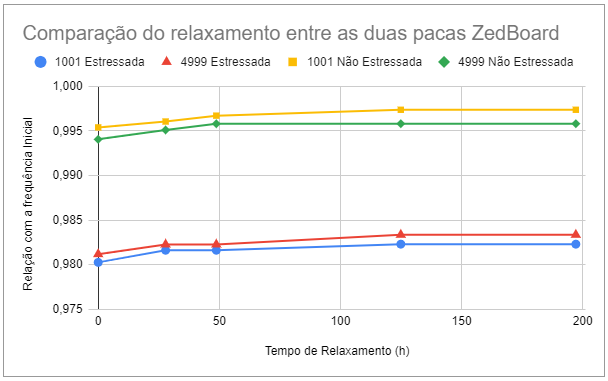
\includegraphics[scale=0.75]{figures/Resultados/RelaxZedBoard}
    \caption{Curva de relaxamento das placas ZedBoard. Fonte: O Autor}
    \label{fig:RelaxZedBoard}
\end{figure}

A Tabela \ref{tab:Relax} mostra o percentual da frequência inicial que foi recuperado durante o período de relaxamento. A proporção da frequência inicial que foi recuperada foi semelhante para todos os osciladores de ambas as Zedboards, já para os osciladores da DE2 houve uma diferença considerável.

\begin{table}[H]
\centering
\caption{Frequência recuperada.}
\begin{tabular}{l|cccc|}
\cline{2-5}
 & \multicolumn{4}{c|}{\textbf{Recuperação (\%)}} \\ \cline{2-5} 
 & \multicolumn{2}{c|}{\textbf{Altera DE2}} & \multicolumn{2}{c|}{\textbf{ZedBoard}} \\ \cline{2-5} 
 & \multicolumn{1}{c|}{\textbf{1001}} & \multicolumn{1}{c|}{\textbf{4999}} & \multicolumn{1}{c|}{\textbf{1001}} & \textbf{4999} \\ \hline
\multicolumn{1}{|l|}{\textbf{Estressados}} & \multicolumn{1}{c|}{0,72} & \multicolumn{1}{c|}{0,74} & \multicolumn{1}{c|}{0,20} & 0,22 \\ \hline
\multicolumn{1}{|l|}{\textbf{Não Estressados}} & \multicolumn{1}{c|}{0,51} & \multicolumn{1}{c|}{0,51} & \multicolumn{1}{c|}{0,20} & 0,17 \\ \hline
\end{tabular}
\label{tab:Relax}
\end{table}

Mas esses valores não refletem exatamente a realidade sobre a recuperação, pois a porcentagem de degradação foi diferente entre as placas. Uma análise mais condizente seria ver a proporção entre a porcentagem da recuperação e a porcentagem da degradação, de forma que se tem a um proporção de quanto da degradação foi recuperada. A Tabela \ref{tab:RelaxProp} mostra esses valores.

\begin{table}[H]
\centering
\caption{Porcentagem da degradação que foi recuperada.}
\begin{tabular}{l|cccc|}
\cline{2-5}
 & \multicolumn{4}{c|}{\textbf{Proporção Recuperada (\%)}} \\ \cline{2-5} 
 & \multicolumn{2}{c|}{\textbf{Altera DE2}} & \multicolumn{2}{c|}{\textbf{ZedBoard}} \\ \cline{2-5} 
 & \multicolumn{1}{c|}{\textbf{1001}} & \multicolumn{1}{c|}{\textbf{4999}} & \multicolumn{1}{c|}{\textbf{1001}} & \textbf{4999} \\ \hline
\multicolumn{1}{|l|}{\textbf{Estressados}} & \multicolumn{1}{c|}{81,25} & \multicolumn{1}{c|}{77,14} & \multicolumn{1}{c|}{10,34} & 11,54 \\ \hline
\multicolumn{1}{|l|}{\textbf{Não Estressados}} & \multicolumn{1}{c|}{81,82} & \multicolumn{1}{c|}{78,26} & \multicolumn{1}{c|}{42,86} & 29,41 \\ \hline
\end{tabular}
\label{tab:RelaxProp}
\end{table}

Nela fica claro que as DE2 tiveram valores de recuperação semelhantes e que ambas recuperaram uma porção considerável, de entorno de 80\%, do que foi degradado. Já as ZedBoards que foram estressadas recuperaram apenas 10\% do que foi degradado e, diferente do outro modelo de FPGA, não teve semelhança com sua contraparte não estressada, que tiveram entre 29\% e 43\% de recuperação. 


